\section{Dati con Intervalli}

Devi utilizzare questa sezione solo quando hai dei dati divisi in
\textbf{Intervalli}, devi anche fare attenzione che il \textbf{numero di
    osservazioni $n > 30$}!!\\

Calcoli da effettuare:

\begin{enumerate}
    \item Riportare i dati in una tabella in Calc:
          \begin{itemize}
              \item \textit{Colonna 1}: $categorie$, probabilmente devi
                    aggiungerle tu, parti da 0 in poi
              \item \textit{Colonna 2}: $intervallo$, del tipo $x_1 - x_2$.
                    Fai sempre attenzione che $x_2 \ge x_1$ !!! In caso li
                    inverti.
              \item  \textit{Colonna 3}: $frequenza$ $f_i$
          \end{itemize}
    \item Aggiungere \textit{Colonna $x_1$} (intervallo più piccolo)
    \item Aggiungere \textit{Colonna $x_2$} (intervallo più grande)
    \item Aggiungere media tra \textit{$x_2$} e \textit{$x_1$}
    \item Calcolare:
          \begin{enumerate} %TODO: potremmo dare un nome (tipo phi) ad ognuna di queste
              \item frequenza pesata = $media_{intervalli} * f_i$
              \item $n$ = $\sum(\text{frequenze})$
              \item media = $\sum(\text{frequenze pesate})/n$
              \item differenza medie = $(media_{intervalli} - media)^2$
              \item frequenza pesata 2 = $\text{differenza medie} * f_i$
              \item frequenza relativa = $f_i * n$
              \item capire la distribuzione se non è data. %TODO: aggiungere ref.
              \item \st{$f(i) = f_i / n$: non serve} %TODO: sbarrare
              \item $p(i)$ = calcolare secondo la distribuzione %TODO: aggiustare
              \item $F_i = n * p(i)$: numero di intervalli unitari teorici
                    con $i$ arrivi
              \item $G_i = \frac{(f_i - F_i)^2}{F_i}$
              \item $V = \sum G_i$: sommare tutti i valori di $G$
              \item $df = \text{Numero Categorie} - 1 - \text{Numero
                            Parametri Distribuzione}$
          \end{enumerate}
    \item Raggruppare le categorie se $\exists \ categoria < 5$: %TODO: agli intervalli succede qualcosa ??
          \begin{itemize}
              \item Parti dall'ultimo a salire (dal basso verso l'alto delle
                    categorie)
              \item Raggruppale tutte nell'ultima categoria che le faccia
                    diventare maggiori di 5 sommando le frequenze.
              \item \textit{Esempio}:
                    \begin{figure}[H]
                        \centering
                        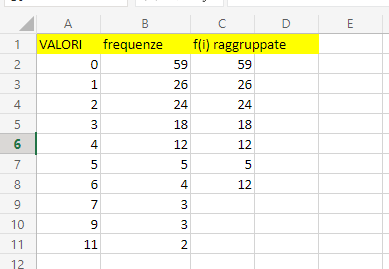
\includegraphics[width=6cm, keepaspectratio]{capitoli/goodnes_of_fit/imgs/vesceragay.png}
                        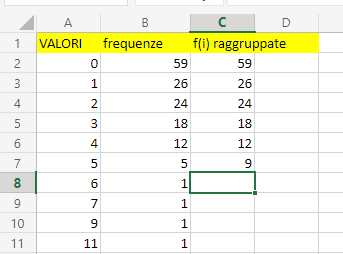
\includegraphics[width=5.5cm, keepaspectratio]{capitoli/goodnes_of_fit/imgs/POSTAMOLTOGAY.png}
                    \end{figure}
          \end{itemize}


\end{enumerate}